\documentclass[12pt]{article}
\usepackage[letterpaper, margin=1in]{geometry}
\usepackage{graphicx}
\usepackage{amsmath}
\usepackage[framed, numbered]{matlab-prettifier}
\lstset{inputpath=../Matlab}
\graphicspath{{../Figures/}}
\title{ELECENG 3TP3 Lab 4}
\author{Raeed Hassan \\ hassam41 \\ McMaster University}
\begin{document}
\maketitle
\pagebreak
\section*{Part 1}
\begin{enumerate}
    \setcounter{enumi}{1}
    \item I hear a constant high frequency sound that plays for 10 seconds.
    \item The MATLAB code used to generate a plot of the first 5 seconds of the waveform is shown in Listing~\ref{listing:p1q3}. The plot of the first five seconds is shown in Figure~\ref{fig:p1q3}.
    \lstinputlisting[style=Matlab-editor, caption={Generating plot of waveform}, label={listing:p1q3}]{part1q3.m}
    \begin{figure}[ht]
        \centering
        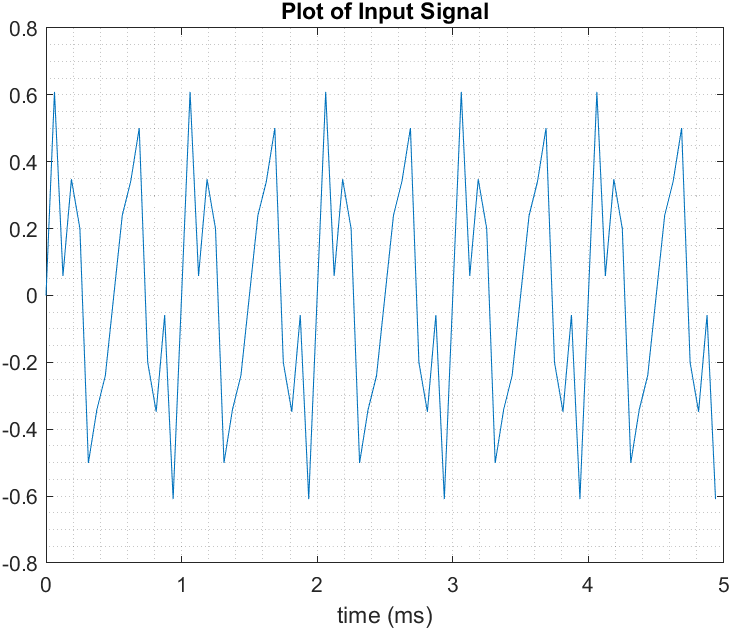
\includegraphics[width=0.7\textwidth]{part1q3.png}
        \caption{\label{fig:p1q3}Plot of first 5 milliseconds of waveform for tones2020.wav}
    \end{figure}
    \item In the plot of the input signal, we can see that there is a periodic signal that repeats every 1 millisecond (frequency of 1000 Hz). It is difficult to tell how many sinusoids make up the signal and their frequencies from the plot of the input signal. The number of sinusoids that make up the signal and their frequencies can be determined by applying the Fourier transform on the input signal.

    \item The plot of the DFT of the audio signal is shown in Figure~\ref{fig:p1q5}. The MATLAB code used to generate the graphs is shown in Listing~\ref{listing:p1q5}.
    \begin{figure}[ht]
        \centering
        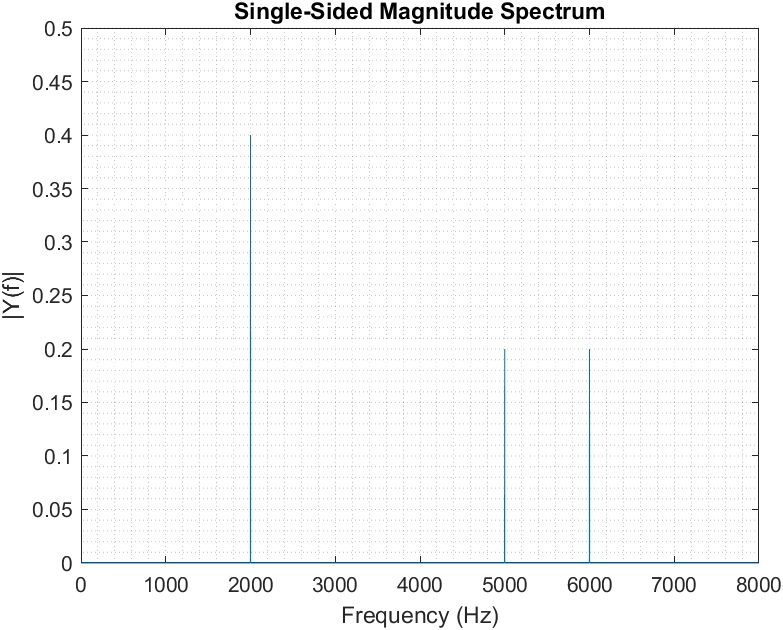
\includegraphics[width=0.55\textwidth]{part1q5.png}
        \caption{\label{fig:p1q5}DFT of the audio signal}
    \end{figure}
    \lstinputlisting[style=Matlab-editor, caption={DFT of the audio signal}, label={listing:p1q5}]{part1q5.m}

    \item The audio signal is made up of three sinusoids, and the frequencies and magnitudes of the sinusoids are: 2000 Hz and 0.4, 5000 Hz and 0.2, and 6000 Hz and 0.2.

    \item The MATLAB code to generate the signal, and compare the plots of the generated signal and the input signal is shown in Listing~\ref{listing:p1q7}. The two plots are shown in Figure~\ref{fig:p1q7}. The plot of the generated signal is identical to the plot of the input signal found in Part 3, which is expected as there is no noise in the input signal (as seen in Part 5) and the input signal is made entirely of the sum of the three determined sinusoids.
    \lstinputlisting[style=Matlab-editor, caption={Generating signal from sinuosoids}, label={listing:p1q7}]{part1q7.m}
    \begin{figure}[ht]
        \centering
        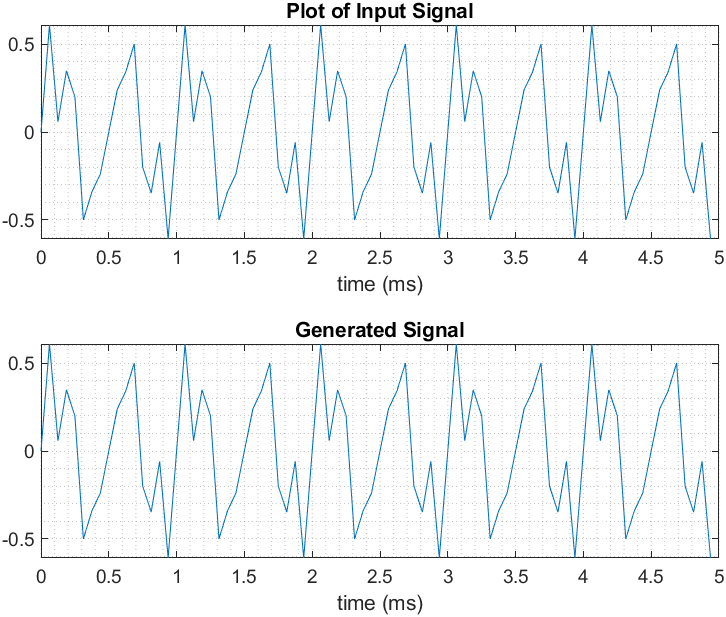
\includegraphics[width=0.6\textwidth]{part1q7.png}
        \caption{\label{fig:p1q7}Comparison of two plots}
    \end{figure}

\end{enumerate}
\newpage
\section*{Part 2}
\begin{enumerate}
    \setcounter{enumi}{1}
    \item The signal is a very noisy sound, that changes to a slightly different tone every second. This behaviour of having a slightly difference tone every second persists for the entire signal.

    \item The single-sided magnitude of the DFT was plotted using the same procedure described in Part I. We can determine the frequencies used in the signal by looking at the plot of the DFT shown in Figure~\ref{fig:p2q3}. The frequencies used in the signal are: 1000 Hz, 2000 Hz, 3000 Hz, 4000 Hz, 5000 Hz, 6000 Hz, 7000 Hz, and 8000 Hz. The MATLAB code used to generate the DFT and save it to a file is shown in Listing~\ref{listing:p2q3}.
    \begin{figure}[ht]
        \centering
        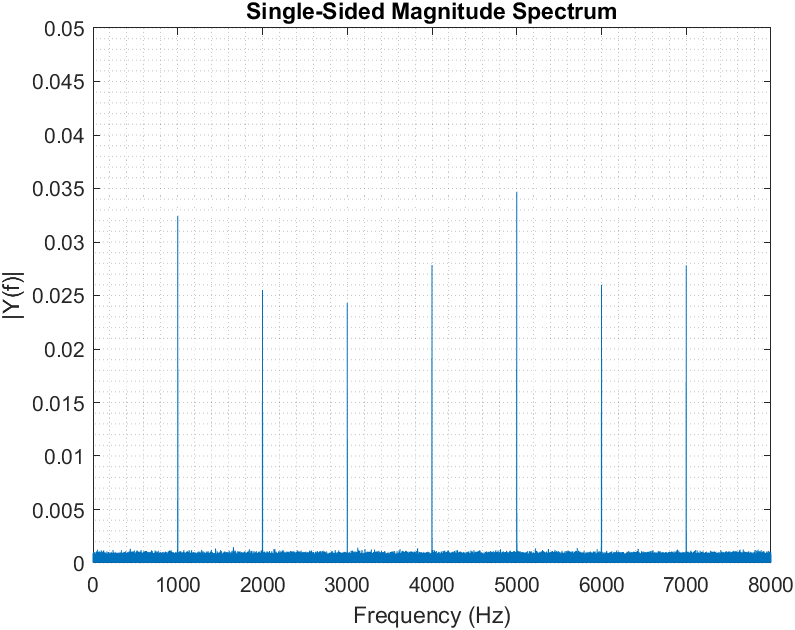
\includegraphics[width=\textwidth]{part2q3.png}
        \caption{\label{fig:p2q3}The DFT of the SecretMessage2020.wav file}
    \end{figure}
    \lstinputlisting[style=Matlab-editor, caption={Generate DFT of SecretMessage2020.wav file}, label={listing:p2q3}]{part2q3.m}

    \item To decode the message, the signal was split up to each of its 1-second symbol periods in a loop, and the FFT of each symbol period was taken. The frequencies present in each period were determined using the maxk function, returning the indices (frequencies) of the four maximum values (maximum magnitudes) in the FTT. The frequencies were put into a 64 x 4 matrix, with each row containing the sorted 4 frequencies present in each of the 64 symbol periods. The MATLAB code used for this is shown in Listing~\ref{listing:p2q4freq}.
    \lstinputlisting[style=Matlab-editor, caption={Determing frequencies contained in each symbol period}, label={listing:p2q4freq}]{part2q4.m}
    The sorted frequencies are matched to the frequencies in the CodeBook.pdf file to decode and generate the message in the signal. A snippet of the MATLAB to perform this is shown in Listing~\ref{listing:p2q4decode}. The decoded message is: "IT DOES NOT MATTER HOW SLOWLY YOU GO AS LONG AS YOU DO NOT STOP."
    \lstinputlisting[style=Matlab-editor, lastline = 13, caption={Matching frequency vectors with message characters to decode message}, label={listing:p2q4decode}]{part2q4decode.m}
\end{enumerate}
\end{document}